%%%%%%%%%%%%%%%%%%%%%%%%%%%%%%%%%%%%%%%%%%%%%%%%%%%%%%%%%%%%%%%%%%%%%%%%%%%%%%%%%%
\begin{frame}[fragile]\frametitle{}
\begin{center}
{\Large Introduction}
\end{center}
\end{frame}

%%%%%%%%%%%%%%%%%%%%%%%%%%%%%%%%%%%%%%%%%%%%%%%%%%%%%%%%%%%
\begin{frame}[fragile]\frametitle{What Makes an AI Agent Different?}
      \begin{itemize}
        \item Unlike LLMs that just respond to prompts, agents are autonomous
        \item Can look at their environment and analyze the situation
        \item Make comprehensive plans to achieve specific goals
        \item Actually take action to execute those plans
        \item Agents bridge the gap between answering and doing
      \end{itemize}
\end{frame}

%%%%%%%%%%%%%%%%%%%%%%%%%%%%%%%%%%%%%%%%%%%%%%%%%%%%%%%%%%%
\begin{frame}[fragile]\frametitle{Welcome to AI Agents}
      \begin{itemize}
        \item AI agents represent one of the most exciting frontiers in AI
        \item Not just everyday chatbots - systems that reason, plan, and take action
        \item Move beyond AI that just answers questions to AI that does things
        \item Can take on complex multi-step tasks autonomously
        \item The core promise: AI that accomplishes goals independently
        \item Technology is advancing rapidly from conversational to agentic AI
      \end{itemize}
\end{frame}


%%%%%%%%%%%%%%%%%%%%%%%%%%%%%%%%%%%%%%%%%%%%%%%%%%%%%%%%%%%
\begin{frame}[fragile]\frametitle{The Impossible Job}
      \begin{itemize}
        \item If your boss tasks you with planning a massive get-together
        \item Must research a huge guest list and plan fancy menu
        \item Needs to find entertainment for the event
        \item A simple chatbot cannot handle these complex requirements
        \item You need an AI agent, not just responses, but actions
        \item Perfect example of why we need more than conversational AI
      \end{itemize}
\end{frame}


%%%%%%%%%%%%%%%%%%%%%%%%%%%%%%%%%%%%%%%%%%%%%%%%%%%%%%%%%%%%%%%%%%%%%%%%%%%%%%%%%%
\begin{frame}[fragile]\frametitle{Introduction to AI Agents}
    \begin{itemize}
        \item 2025 is expected to be the year of AI agents.
        \item AI agents combine multiple components to solve complex problems.
        \item Shifting from monolithic models to compound AI systems.
        \item Compound AI systems use system design for better problem solving.
        \item AI agents improve with reasoning, acting, and memory components. (ReAct = Reasoning + Acting)
    \end{itemize}
\end{frame}


%%%%%%%%%%%%%%%%%%%%%%%%%%%%%%%%%%%%%%%%%%%%%%%%%%%%%%%%%%%%%%%%%%%%%%%%%%%%%%%%%%
\begin{frame}[fragile]\frametitle{The Evolution of AI Capabilities}
\begin{itemize}
    \item \textbf{Traditional Programming:} Needed code to operate
    \item \textbf{Traditional ML:} Needed feature engineering
    \item \textbf{Deep Learning:} task-specific model
    \item \textbf{ChatGPT (2022):} Many tasks single model
    \begin{itemize}
        \item Zero-shot learning (no examples needed)
        \item In-context learning (understands from instructions)
    \end{itemize}
    \item \textbf{Agents (2024 \ldots):} Can actually \textbf{do things}, not just talk
\end{itemize}
\end{frame}

%%%%%%%%%%%%%%%%%%%%%%%%%%%%%%%%%%%%%%%%%%%%%%%%%%%%%%%%%%%%%%%%%%%%%%%%%%%%%%%%%%
\begin{frame}[fragile]\frametitle{Why Does ``Taking Action'' Matter?}
\begin{itemize}
    \item In 2022, ChatGPT was revolutionary because AI felt conversational
    \item By 2024, people wanted more than conversation, they wanted \textbf{execution}
    \item Examples of what users now expect:
    \begin{itemize}
        \item Instead of listing leads ? \textbf{email them directly}
        \item Instead of summarizing docs ? \textbf{file and create workflow tasks}
        \item Instead of suggesting products ? \textbf{customize landing pages}
    \end{itemize}
    \item This shift from \textbf{information} to \textbf{action} defines the agent era
\end{itemize}
\end{frame}


%%%%%%%%%%%%%%%%%%%%%%%%%%%%%%%%%%%%%%%%%%%%%%%%%%%%%%%%%%%%%%%%%%%%%%%%%%%%%%%%%%
\begin{frame}[fragile]\frametitle{How Agents Work?}
    \begin{itemize}
        \item Agent acts, take you from one state to the other state, provides value by workflow automation. (ReAct paper: Reasoning and Action), it can plan and make decisions.
		\item Agents have access to tools (ToolFormer paper) e.g. Search APIs, booking, send email etc.
		\item Interacting of external environment and other Agents, etc.
		\item Memory to keep the history of conversations/actions done so far.
		\item May have human-in-loop to keep it sane in the wild-world.
		\item Agents were there from 1950's but they are effective because of LLMs.
        \item Agents are systems where LLMs dynamically direct their own processes and tool usage
        \item Can operate autonomously over extended periods using various tools
        \item Distinct from workflows: agents have dynamic control vs. predefined code paths
        \item Essential component in modern AI systems with varying degrees of autonomy
    \end{itemize}
\end{frame}

%%%%%%%%%%%%%%%%%%%%%%%%%%%%%%%%%%%%%%%%%%%%%%%%%%%%%%%%%%%
\begin{frame}[fragile]\frametitle{The Agent's Fundamental Game Loop}
      \begin{itemize}
        \item Not a one-and-done action, but a continuous reasoning loop
        \item Similar to a programming while loop that keeps iterating
        \item \textbf{Thought}: Analyzes situation and plans next step
        \item \textbf{Action}: Calls specific tools to execute the plan
        \item \textbf{Observation}: Examines results of the action taken
        \item Cycle repeats: Thought → Action → Observation
        \item Continues until the task is completely accomplished
        \item This loop enables continuous adaptation and problem-solving
      \end{itemize}
\end{frame}

%%%%%%%%%%%%%%%%%%%%%%%%%%%%%%%%%%%%%%%%%%%%%%%%%%%%%%%%%%%
\begin{frame}[fragile]\frametitle{Agent's Inner Monologue}
      \begin{itemize}
        \item Agents have visible thought processes before taking action
        \item Example: ``User wants weather in New York. I have a tool for that''.
        \item ``My first move is to call the weather API''.
        \item Internal planning step makes agents more than reactive programs
        \item Reasoning through problems before execution
        \item This deliberation distinguishes agents from simple scripts
        \item Shows intelligent decision-making rather than blind execution
      \end{itemize}
\end{frame}

%%%%%%%%%%%%%%%%%%%%%%%%%%%%%%%%%%%%%%%%%%%%%%%%%%%%%%%%%%%%%%%%%%%%%%%%%%%%%%%%%%
\begin{frame}[fragile]\frametitle{How Do Agents Take Action?}
\begin{itemize}
    \item The magic lies in \textbf{tools} and \textbf{function calling}
    \item Agents are paired with APIs, plugins, or external systems
    \item Instead of just text responses, LLMs output structured commands:
    \begin{itemize}
        \item ``Call the send\_email() function with these inputs...''
        \item ``Fetch records from CRM using this query...''
        \item ``Schedule a meeting for Tuesday at 2PM...''
    \end{itemize}
    \item \textbf{Mental model:} LLM = brain, Tools = hands
    \item Without tools, agents just talk. With tools, they act.
\end{itemize}
\end{frame}


%%%%%%%%%%%%%%%%%%%%%%%%%%%%%%%%%%%%%%%%%%%%%%%%%%%%%%%%%%%
\begin{frame}[fragile]\frametitle{Defining AI Agents with an example}

      \begin{itemize}
		\item Planning a trip involves many complex tasks
		\item Point A: Just discussing the trip
		\item Point B: All bookings and itinerary ready
		\item AI Agents aim to take you from A to B
		\item First idea: Agent adds value by saving time/money
      \end{itemize}

		\begin{center}
		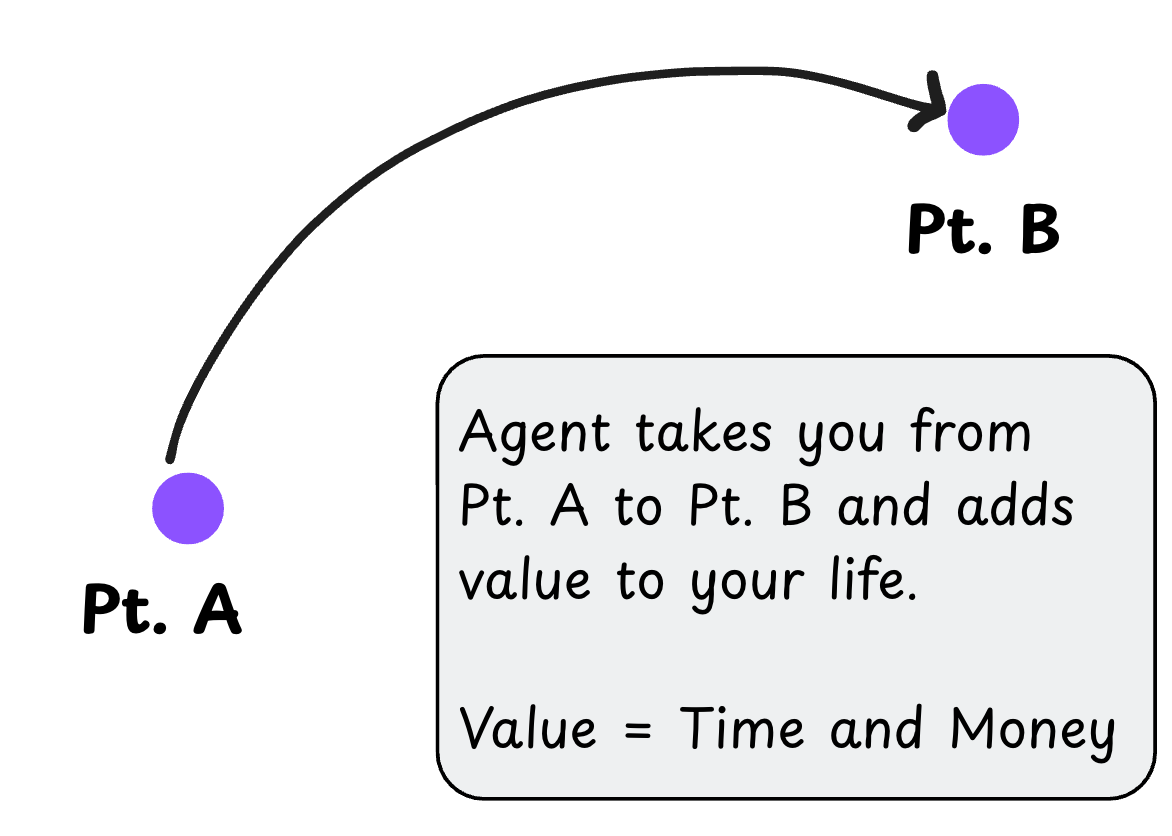
\includegraphics[width=0.6\linewidth,keepaspectratio]{aiagents25}
		
		{\tiny (Ref: Vizuara AI Agents Bootcamp)}
		\end{center}	

\end{frame}

%%%%%%%%%%%%%%%%%%%%%%%%%%%%%%%%%%%%%%%%%%%%%%%%%%%%%%%%%%%
\begin{frame}[fragile]\frametitle{Evolving Definition of Agents}

      \begin{itemize}
		\item Not all tools from A to B are agents (e.g., cars)
		\item Agents must plan and make decisions
		\item Second definition includes decision-making ability
		\item Example: Choosing flights based on budget
		\item Planning daily itinerary needs contextual judgment
      \end{itemize}

		\begin{center}
		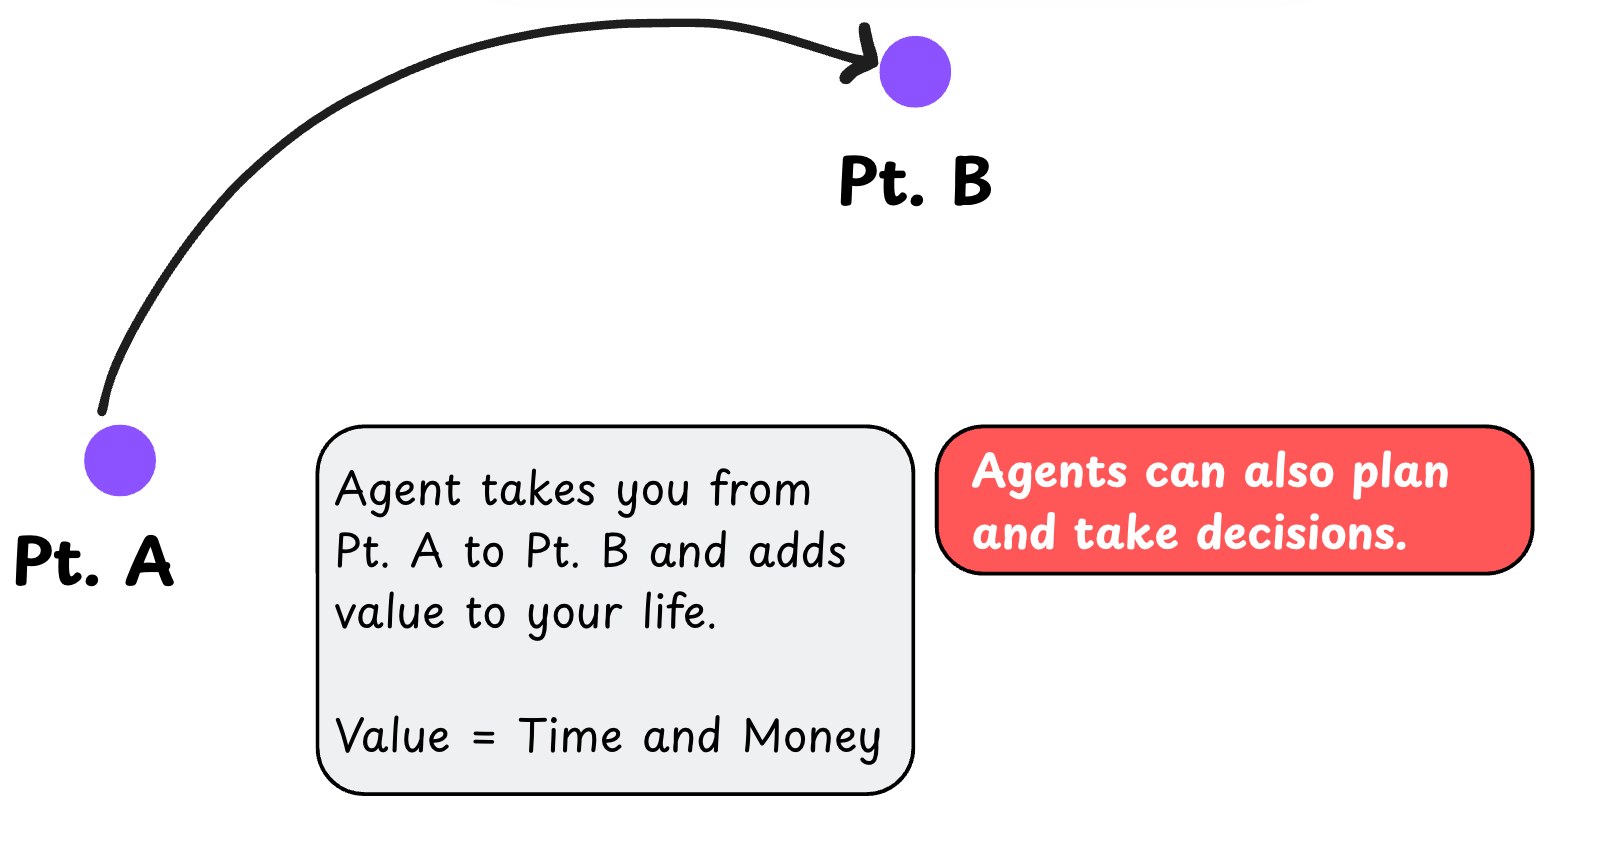
\includegraphics[width=0.6\linewidth,keepaspectratio]{aiagents26}
		
		{\tiny (Ref: Vizuara AI Agents Bootcamp)}
		\end{center}	

\end{frame}

%%%%%%%%%%%%%%%%%%%%%%%%%%%%%%%%%%%%%%%%%%%%%%%%%%%%%%%%%%%
\begin{frame}[fragile]\frametitle{Agents Need Tools}

      \begin{itemize}
        \item Even self-driving cars plan but are not agents
        \item Agents need access to external tools
        \item Tools = Access to services (e.g., Gmail, Booking)
        \item Agents perform tasks using these tools
        \item Third definition adds tool access to capabilities
      \end{itemize}

		\begin{center}
		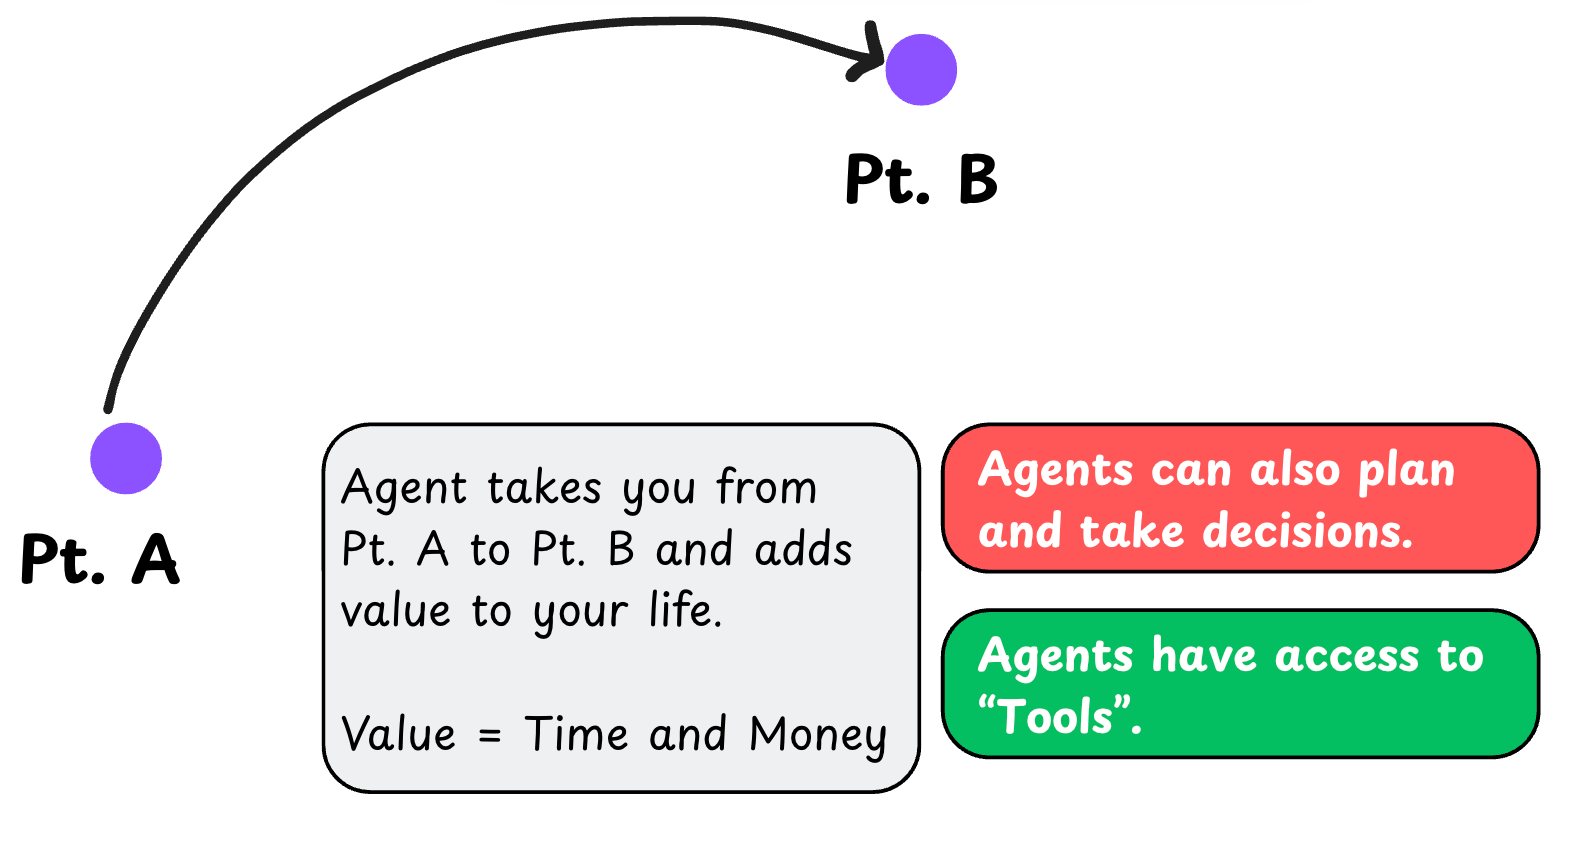
\includegraphics[width=0.6\linewidth,keepaspectratio]{aiagents27}
		
		{\tiny (Ref: Vizuara AI Agents Bootcamp)}
		\end{center}	

\end{frame}

%%%%%%%%%%%%%%%%%%%%%%%%%%%%%%%%%%%%%%%%%%%%%%%%%%%%%%%%%%%
\begin{frame}[fragile]\frametitle{Rise of LLMs in Agents}

      \begin{itemize}
        \item Transformers (2017) enabled powerful LLMs
        \item LLMs understand and generate human language
        \item Agents use LLMs for reasoning and planning
        \item LLMs enable understanding of webpages and writing emails
        \item Fourth definition: Agents are LLMs with tools and planning ability
      \end{itemize}

		\begin{center}
		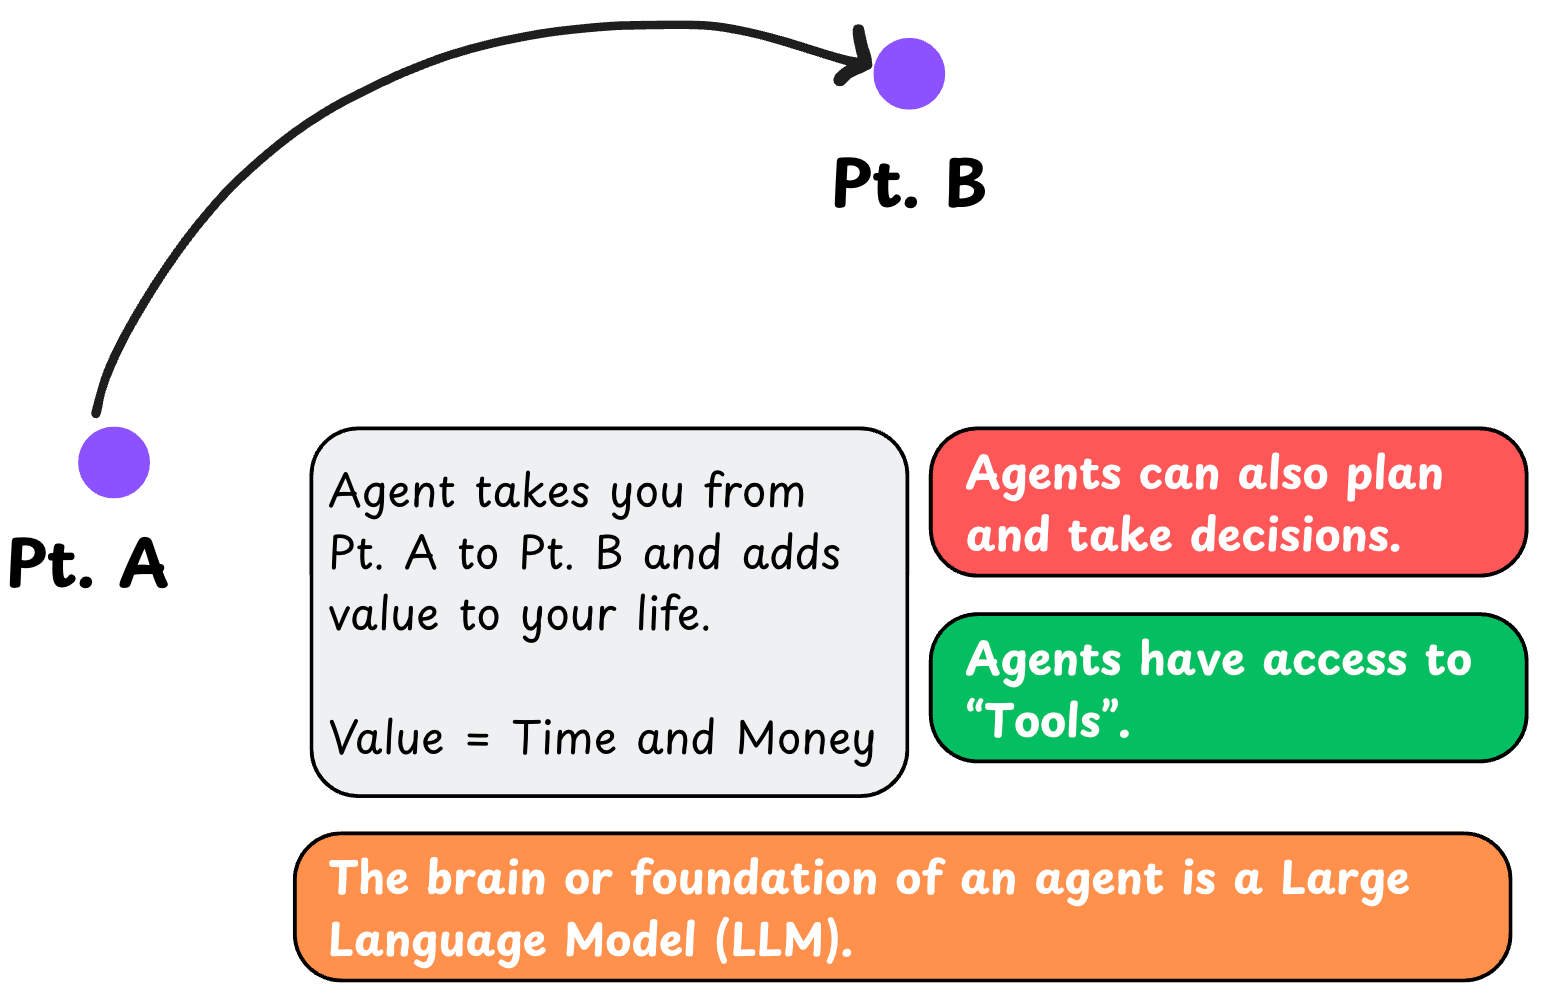
\includegraphics[width=0.6\linewidth,keepaspectratio]{aiagents28}
		
		{\tiny (Ref: Vizuara AI Agents Bootcamp)}
		\end{center}	

\end{frame}



%%%%%%%%%%%%%%%%%%%%%%%%%%%%%%%%%%%%%%%%%%%%%%%%%%%%%%%%%%%%%%%%%%%%%%%%%%%%%%%%%%
\begin{frame}[fragile]\frametitle{What Is an Agent? (Technical Definition)}
\begin{itemize}
    \item Agent acts and takes you from one state to another, providing value through workflow automation
    \item Based on ReAct paradigm: \textbf{Reasoning + Acting}
    \item Key capabilities:
    \begin{itemize}
        \item Can plan and make decisions
        \item Has access to tools (search APIs, booking, email, etc.)
        \item Interacts with external environments and other agents
        \item Maintains memory of conversations and actions
        \item May include human-in-the-loop for safety
    \end{itemize}
    \item Agents existed since the 1950s but are now effective because of LLMs
\end{itemize}
\end{frame}


%%%%%%%%%%%%%%%%%%%%%%%%%%%%%%%%%%%%%%%%%%%%%%%%%%%%%%%%%%%%%%%%%%%%%%%%%%%%%%%%%%
\begin{frame}[fragile]\frametitle{Two Ways to Define Agents}
\begin{columns}
    \begin{column}[T]{0.5\linewidth}
        \textbf{Technical View:}
        \begin{itemize}
            \item LLM (brain)
            \item + Tools (hands)
            \item + Planning (strategy)
            \item + Memory (context)
            \item + State management
        \end{itemize}
    \end{column}
    \begin{column}[T]{0.5\linewidth}
        \textbf{Business View:}
        \begin{itemize}
            \item Systems that complete tasks end-to-end
            \item Focus on outcomes, not components
            \item Solve real-world problems
            \item Provide measurable value
        \end{itemize}
    \end{column}
\end{columns}

\vspace{0.5cm}
\textbf{Important:} Today's agents are \textbf{engineering wrappers} around AI models, the intelligence comes from the LLMs, agents help act on that intelligence.
\end{frame}


%%%%%%%%%%%%%%%%%%%%%%%%%%%%%%%%%%%%%%%%%%%%%%%%%%%%%%%%%%%
\begin{frame}[fragile]\frametitle{Final Definition of Agents}

      \begin{itemize}
        \item Agents can learn from feedback and environment
        \item Agents interact with tools, humans, and websites
        \item They improve with experience (memory)
        \item Fifth definition: LLMs + Tools + Planning + Learning
        \item Agents evolve over time via memory and feedback
      \end{itemize}

		\begin{center}
		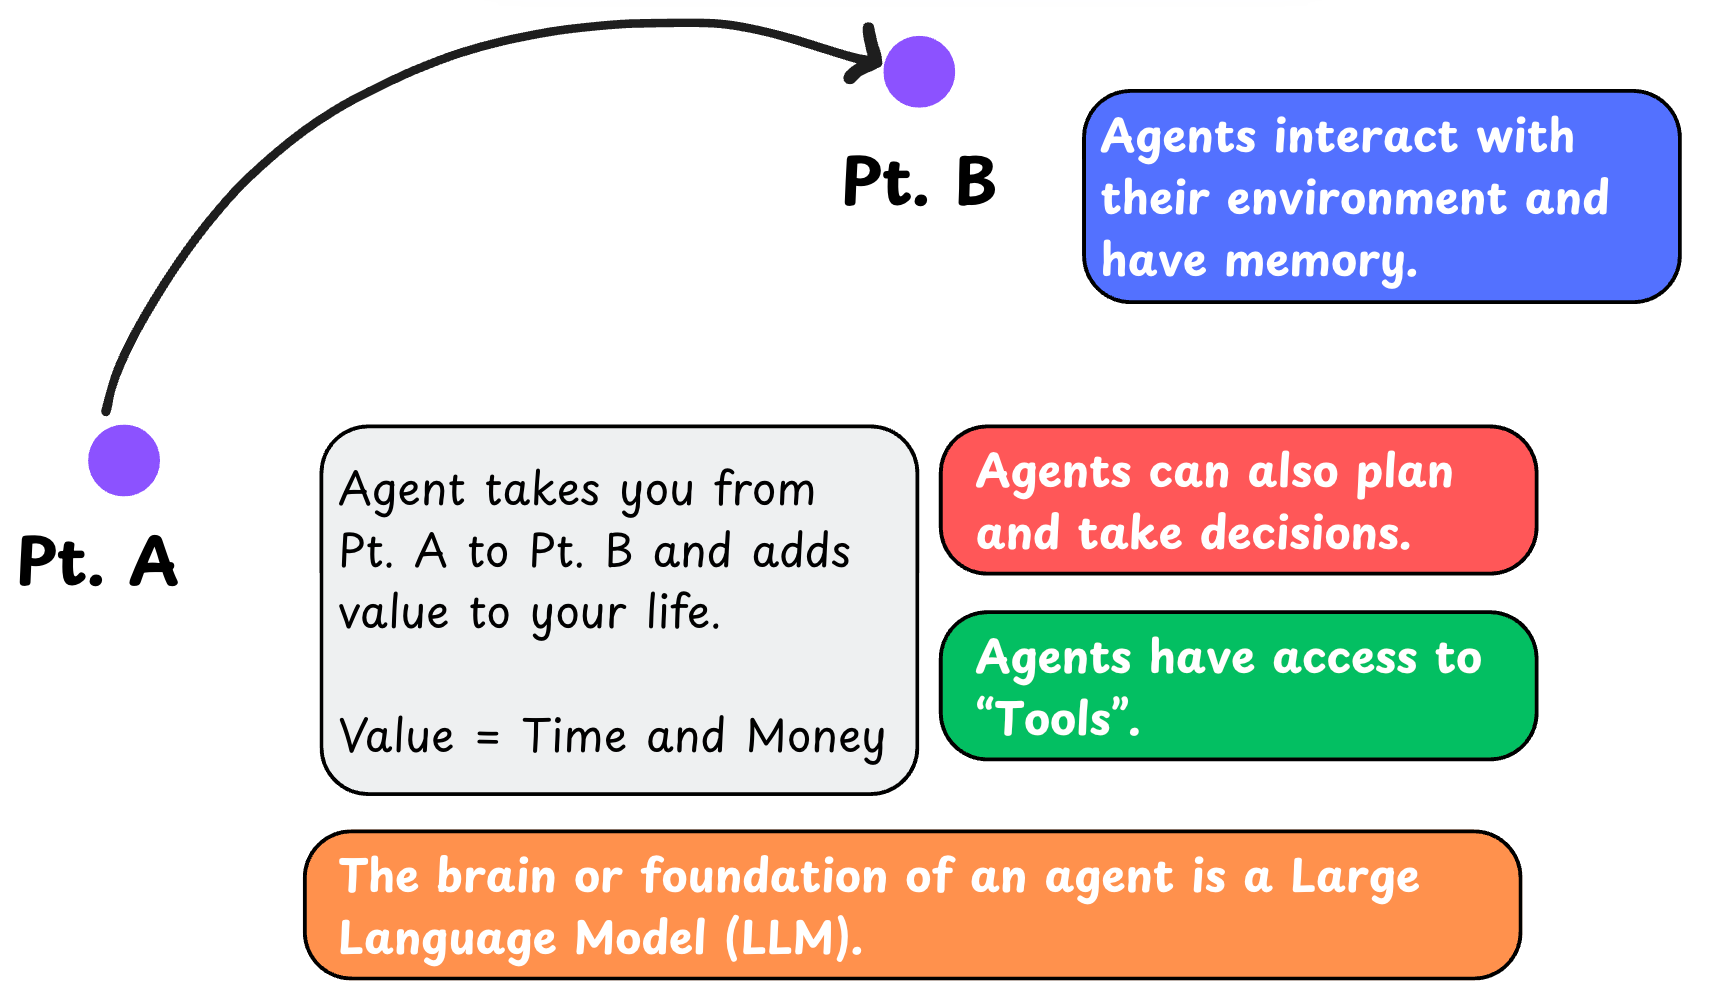
\includegraphics[width=0.6\linewidth,keepaspectratio]{aiagents29}
		
		{\tiny (Ref: Vizuara AI Agents Bootcamp)}
		\end{center}	

\end{frame}

%%%%%%%%%%%%%%%%%%%%%%%%%%%%%%%%%%%%%%%%%%%%%%%%%%%%%%%%%%%
\begin{frame}[fragile]\frametitle{Understanding Agency}

      \begin{itemize}
        \item Agency = Level of autonomy an agent has
        \item Low agency → less value
        \item High agency → high value
        \item More autonomous agents can handle complex tasks
        \item Agency is key to measuring agent usefulness
      \end{itemize}

		\begin{center}
		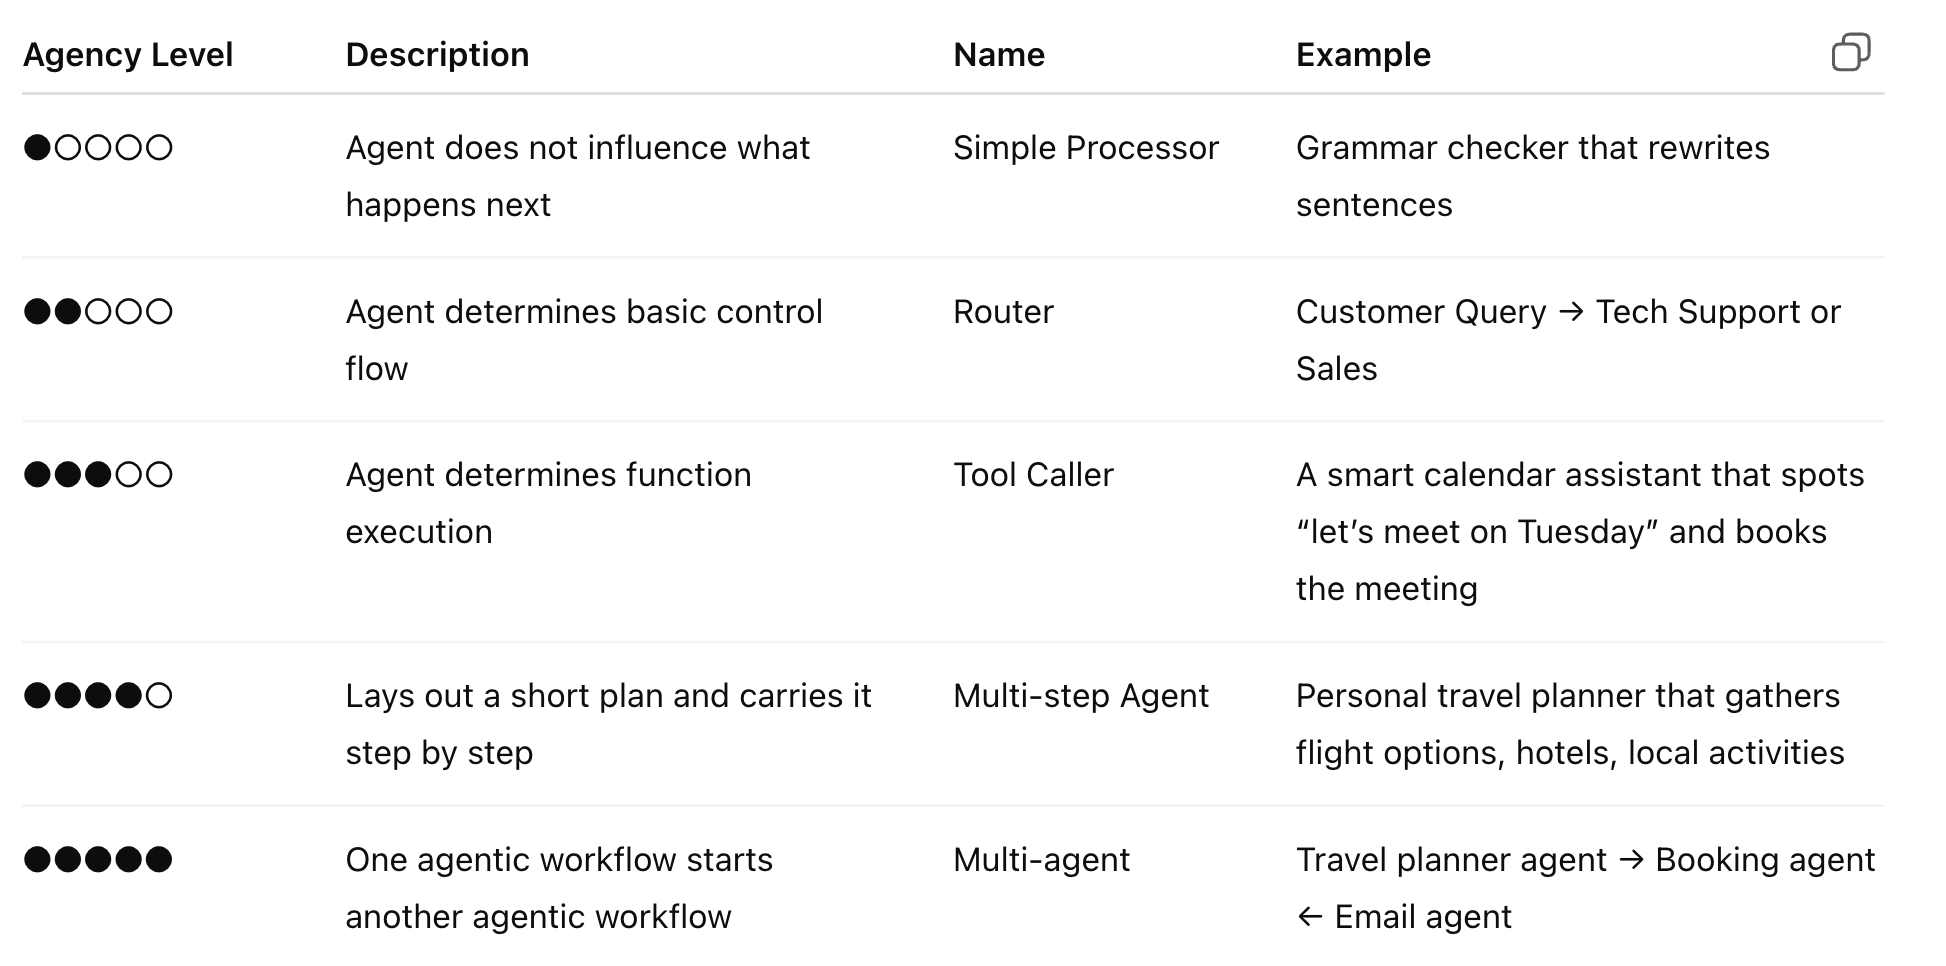
\includegraphics[width=0.8\linewidth,keepaspectratio]{aiagents30}
		
		{\tiny (Ref: Vizuara AI Agents Bootcamp)}
		\end{center}	

\end{frame}

%%%%%%%%%%%%%%%%%%%%%%%%%%%%%%%%%%%%%%%%%%%%%%%%%%%%%%%%%%%
\begin{frame}[fragile]\frametitle{Tools: The Agent's Hands}
      \begin{itemize}
        \item LLM is the agent's brain; tools are its hands
        \item Tools are functions agents call to interact with the world
        \item Can search web, run calculations, or query databases
        \item Bridge between thinking and doing in the real world
        \item Enable agents to move from planning to execution
        \item Without tools, agent thoughts would be useless
        \item Tools provide the interface to external systems and data
      \end{itemize}
\end{frame}

%%%%%%%%%%%%%%%%%%%%%%%%%%%%%%%%%%%%%%%%%%%%%%%%%%%%%%%%%%%
\begin{frame}[fragile]\frametitle{Two Ways Agents Use Tools}
      \begin{itemize}
        \item \textbf{JSON Agent}: Writes structured work orders for other systems
        \item JSON approach requires external system to read and execute
        \item \textbf{Code Agent}: Directly writes and runs code blocks
        \item Code approach is more direct and powerful
        \item Code is naturally more expressive than JSON
        \item Can handle complex logic like loops and conditionals
        \item Modular, easier to debug, and taps into existing libraries
        \item Code agents can access thousands of APIs directly
      \end{itemize}
\end{frame}

%%%%%%%%%%%%%%%%%%%%%%%%%%%%%%%%%%%%%%%%%%%%%%%%%%%%%%%%%%%
\begin{frame}[fragile]\frametitle{Code Agent in Action}
      \begin{itemize}
        \item Alfred needs a gala menu - agent has ``suggest\_menu'' tool
        \item Agent doesn't just make up suggestions randomly
        \item Generates and runs actual code to call the specific tool
        \item Gets real results from the tool execution
        \item Super direct, efficient, and powerful way to take action
        \item Code generation enables precise tool interaction
        \item Results are based on actual tool capabilities, not hallucination
      \end{itemize}
\end{frame}

%%%%%%%%%%%%%%%%%%%%%%%%%%%%%%%%%%%%%%%%%%%%%%%%%%%%%%%%%%%
\begin{frame}[fragile]\frametitle{Advanced Pattern: Agentic RAG}
      \begin{itemize}
        \item Traditional RAG: Retrieval Augmented Generation fetches info before answering
        \item Agentic RAG supercharges this with intelligent multi-step processes
        \item Turns retrieval itself into an agent-driven task
        \item Like having a master researcher on staff
        \item Doesn't just do one search - runs complete research processes
        \item Rewrites queries for better results and runs multiple searches
        \item Uses findings to inform next searches and validates accuracy
        \item Pulls from both private data and public web sources
      \end{itemize}
\end{frame}

%%%%%%%%%%%%%%%%%%%%%%%%%%%%%%%%%%%%%%%%%%%%%%%%%%%%%%%%%%%
\begin{frame}[fragile]\frametitle{Multi-Agent Systems: Digital Teams}
      \begin{itemize}
        \item Complex problems like finding the missing Batmobile need teams
        \item Single agents can't handle web searches, calculations, and visualization
        \item Solution: Build teams of specialized agents
        \item Manager agent acts as project lead breaking down big tasks
        \item Delegates work to specialist agents with specific skills
        \item Web agent handles online searching while manager coordinates
        \item Manager focuses on big picture and final integration
        \item Digital division of labor for complex problem solving
      \end{itemize}
\end{frame}

%%%%%%%%%%%%%%%%%%%%%%%%%%%%%%%%%%%%%%%%%%%%%%%%%%%%%%%%%%%
\begin{frame}[fragile]\frametitle{The GAIA Benchmark Reality Check}
      \begin{itemize}
        \item GAIA benchmark tests real-world multi-step problems
        \item Measures how well systems handle tricky, complex tasks
        \item Results are eye-opening and show current limitations
        \item Humans solve these tasks with 92\% accuracy
        \item Today's most advanced AI models: only 15\% accuracy
        \item Massive 77\% gap between human and AI performance
        \item This gap is exactly what agentic systems aim to close
        \item Shows the enormous potential for improvement
      \end{itemize}
\end{frame}

%%%%%%%%%%%%%%%%%%%%%%%%%%%%%%%%%%%%%%%%%%%%%%%%%%%%%%%%%%%
\begin{frame}[fragile]\frametitle{The Fundamental Shift}
      \begin{itemize}
        \item Moving from conversational AI to agentic AI era
        \item Old paradigm: Ask questions, get answers
        \item New paradigm: State goals, systems plan and accomplish them
        \item Represents fundamental change in human-computer interaction
        \item Technology for building personal AI assistants advancing rapidly
        \item Not a question of ``if'' but ``when'' this becomes reality
        \item The future Alfred is closer than we think
        \item Prepare for AI that can handle ``impossible'' complex tasks
      \end{itemize}
\end{frame}


%%%%%%%%%%%%%%%%%%%%%%%%%%%%%%%%%%%%%%%%%%%%%%%%%%%%%%%%%%%
\begin{frame}[fragile]\frametitle{Papers that Shaped AI Agents}

      \begin{itemize}
        \item Core research papers laid the foundation
        \item Introduced key frameworks and architectures
        \item Sparked recent boom in agent development
        \item Include Transformer and Agentic frameworks
        \item Major driving force in LLM-based agent systems
      \end{itemize}

		\begin{center}
		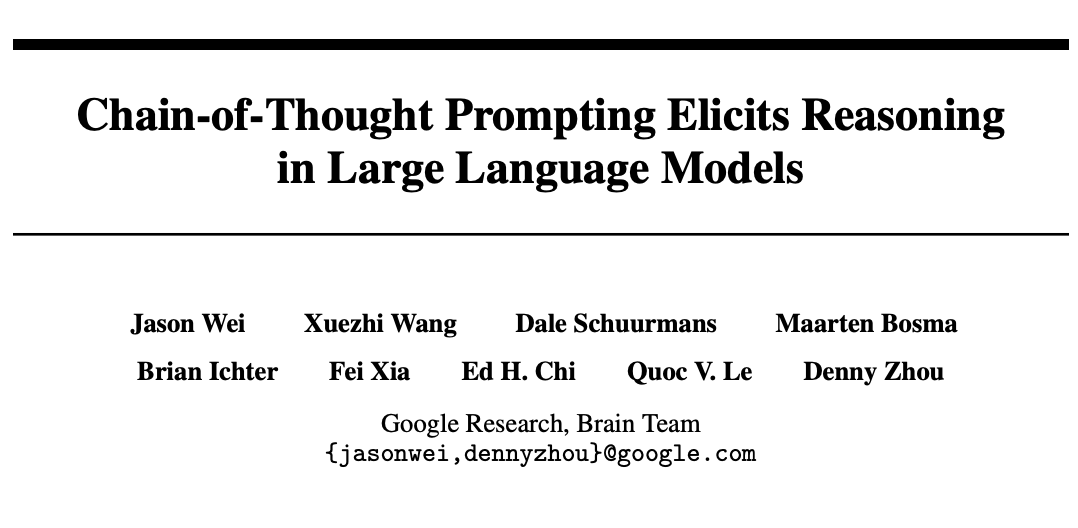
\includegraphics[width=0.45\linewidth,keepaspectratio]{aiagents31}
		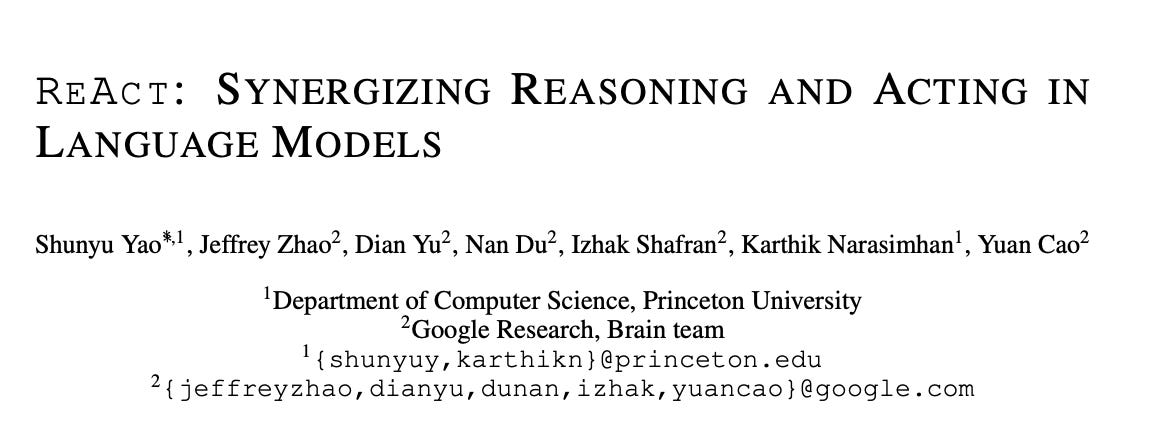
\includegraphics[width=0.45\linewidth,keepaspectratio]{aiagents32}
		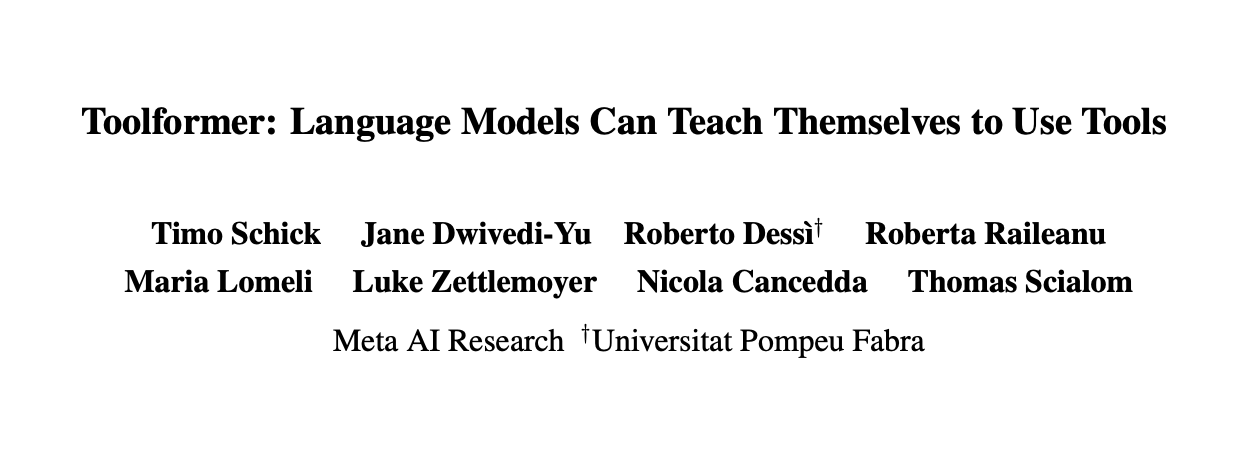
\includegraphics[width=0.45\linewidth,keepaspectratio]{aiagents33}
		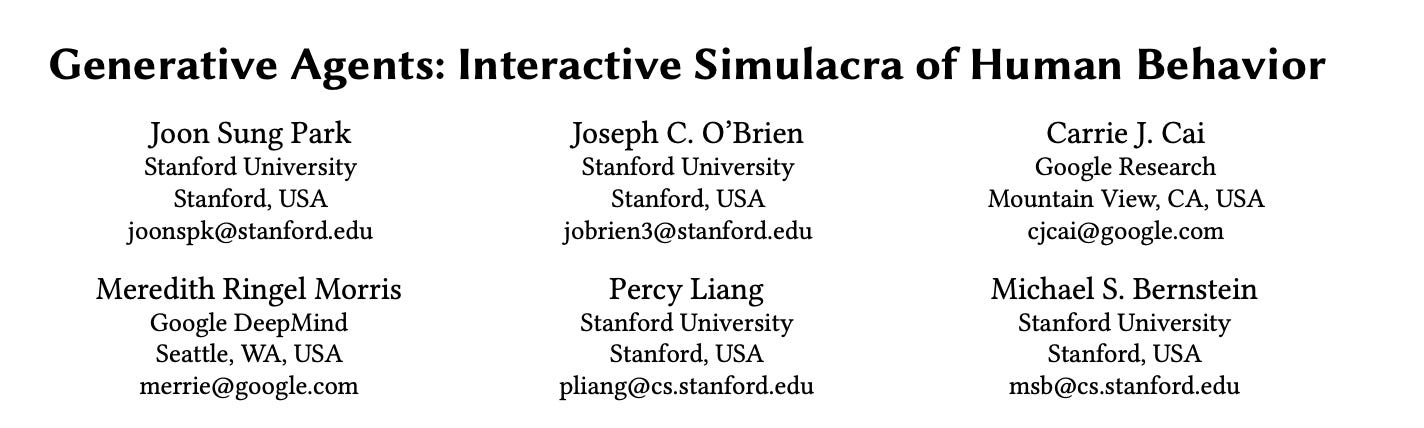
\includegraphics[width=0.45\linewidth,keepaspectratio]{aiagents34}
		
		{\tiny (Ref: Vizuara AI Agents Bootcamp)}
		\end{center}	
 
\end{frame}

%%%%%%%%%%%%%%%%%%%%%%%%%%%%%%%%%%%%%%%%%%%%%%%%%%%%%%%%%%%%%%%%%%%%%%%%%%%%%%%%%%
\begin{frame}[fragile]\frametitle{When to Use Agents?}
    \begin{itemize}
        \item Best suited for tasks requiring flexibility and model-driven decision-making
        \item Consider tradeoffs: agents increase latency and cost for better task performance
        \item Recommended for open-ended problems with unpredictable steps
        \item Simple solutions preferred - single LLM calls with retrieval often sufficient
    \end{itemize}
\end{frame}

%%%%%%%%%%%%%%%%%%%%%%%%%%%%%%%%%%%%%%%%%%%%%%%%%%%%%%%%%%%%%%%%%%%%%%%%%%%%%%%%%%
\begin{frame}[fragile]\frametitle{Future AI Applications}
\begin{itemize}
    \item What are future AI applications like?
    \begin{itemize}
        \item \textbf{Generative:} Generate content like text and images
        \item \textbf{Agentic:} Execute complex tasks on behalf of humans
    \end{itemize}
    \item How do we empower every developer to build them?
    \begin{itemize}
        \item \textbf{Co-Pilots:} Human-AI collaboration
        \item \textbf{Autonomous:} Independent task execution
    \end{itemize}
    \item 2024 is expected to be the year of AI agents
\end{itemize}
\end{frame}

%%%%%%%%%%%%%%%%%%%%%%%%%%%%%%%%%%%%%%%%%%%%%%%%%%%%%%%%%%%
\begin{frame}[fragile]\frametitle{The Big Question}
      \begin{itemize}
        \item Agentic AI technology is moving incredibly fast
        \item Personal AI assistants will soon be capable of complex tasks
        \item Think beyond simple queries to multi-step accomplishments
        \item Consider what ``impossible'' tasks you want to delegate
        \item What complex, party-of-the-century level challenge will you tackle?
        \item The era of AI that truly does rather than just discusses
        \item Prepare for AI assistants that can handle your biggest challenges
      \end{itemize}
\end{frame}


